

\chaptery{A \textsc{html}, \textsc{xhtml} és a \textsc{css}}%
\label{cha:html}

A hálózat elterjedésével lehetővé vált az információk különböző oldalakon
történő tárolása, amelyhez idővel szükségessé vált egy ezt segítő
jelölésrendszer kialakítása. Ezáltal már nem pusztán szöveges információt
lehetett átadni, hanem azt is, hogy ezen szöveg melyik része milyen szerepet
tölt be, ráadásul nagyon könnyen lehetett szerkeszteni az ilyen oldalakat. Ezt
teszi lehetővé a \textsc{html} \cite{html}, amely a 90-es években jelent meg és
terjedt el. A \textsc{html} egy betűszó, a \emph{Hypertext Markup Language}
rövidítése, vagyis egy olyan jelölő nyelv, amely segítségével az oldalak között
lehet lépegetni.

Ma is \textsc{html}-ben készül a legtöbb (web)oldal, azonban már nem statikusak,
valamilyen program készíti el akkor, amikor a felhasználó a böngészője
segítségével lekérdezi. Sőt, a letöltött oldal is dinamikus, hiszen JavaScript
segítségével megváltoztatható az oldal kinézete, vagy éppen az űrlapok mezőit
már a böngészőben le lehet ellenőrizni, hogy a felhasználó tudja, melyiket kell
még javítania. Ma már egyre jobban terjed az a megoldás is, amit szintén
JavaScript-tel oldanak meg, hogy a letöltött oldal egyes részei úgy frissülnek,
hogy egy JavaScript program kérdezi le az adatokat, a felhasználónak nem kell az
oldalt frissítenie, vagy másik oldalra lépnie (\textsc{ajax} \cite{ajax}).

Mára nagyon sok hibás weboldal készült, ahol a szerkezetet jelző címkék
sorrendje helytelen, vagy egyszerűen nincs is. Részben ezt hivatott kiküszöbölni
a \textsc{html} egyik változata, az \textsc{xhtml} \cite{xhtml1,xhtml11}, amely
szigorúan veszi a jelöléseket, ezáltal egy program is könnyebben feldolgozhatja,
és átláthatóbb is.

Az eredeti változatot (\textsc{html 4}) ma is fejlesztik, a következő változatra
elkészült egy javaslat, amely sajnos figyelmen kívül hagyja az \texttt{xhtml}
nyújtotta előnyeket.


\section{A(z \textsc{x})\textsc{html}}

Minden szónál többet ér egy példa, így álljon itt egy példa minimális
\textsc{xhtml} 1.1-es oldalra - amely megfelel a legújabb \textsc{w3c}
ajánlásnak \cite{html}, és \aref{fig:xhtml-minimal}.\ ábrán látható.

\begin{figure}[tbh]\center
\begin{VerbExampleNum}
<?xml version="1.0" encoding="ISO-8859-2"?>
<!DOCTYPE html PUBLIC "-//W3C//DTD XHTML 1.1//EN"
"http://www.w3.org/TR/xhtml11/DTD/xhtml11.dtd">
<html xmlns="http://www.w3.org/1999/xhtml" xml:lang="hu">
<head><title>Ez a cím</title></head>
<body>
Itt van valamilyen szöveg
</body>
</html>
\end{VerbExampleNum}
   \caption{Egy minimális \textsc{xhtml} oldal}
  \label{fig:xhtml-minimal}
\end{figure}


Az első sor jelzi, hogy ez nem csupán egy \textsc{html} oldal, hanem egy olyan
dokumentum,
amely megfelel az XML szabványnak \cite{xml} is. A második és harmadik sor még
mindig nem része magának a \textsc{html} oldalnak, hanem annak szerkezetét
definiálja: azt, hogy hol van a dokumentumtípust leíró definíció, és számos
kapcsolódó információt.

Látható, hogy különböző jelentésű szavak szerepelnek kacsacsőrök
között. Mindegyik ilyen szó egy-egy címke (angolul: tag), amely a dokumentum
szerkezetét határozza meg. Szerepelnek nevek (pl.\ \texttt{html}, \texttt{head},
\texttt{title}), és
a névhez tartozó tulajdonságok is, ilyen például az \texttt{xml:lang}, mely a
dokumentum nyelvét határozza meg. A tulajdonságok vagy attribútumok mindegyike
egy névből, és egy attól egyenlőségjellel elválasztott értékből áll. Az
értékeket idézőjelek közé kell tenni, ugyanis szerepelhet bennük szóköz, és
ezáltal egyértelmű, hogy mettől meddig tartanak.


\section{A \textsc{html} elemek}
Az előzőek figyelembe vételével már könnyen definiálhatóak a \textsc{html} és
\textsc{xhtml} dokumentumok építőkövei, a \textsc{html} elemek (element). Ezek
mindegyike egy névből áll, valamint tulajdonságokból (attributes). A nevet
szokták címkének (tag) hívni. Mindegyiket le kell zárni, vagyis például a
\texttt{html} elemnek van egy nyitó és egy lezáró fele is: \verb|<html>| és
\verb|</html>|; a lezáró rész a nyitóval azonos, azonban csak a nevet
tartalmazza, amelyet egy perjel előz meg.

Az elemek egymásba ágyazhatóak, vagyis majdnem mindig szerepelhet egy másik elem
is bármely másikban, persze vannak kivételek is. A legkülső elem a
\textsc{html}, melyen belül két másiknak kell szerepelnie (két gyereke
van), az első a \texttt{head}, a második a \texttt{body}. Az előbbi az oldal
megjelenítőjének szól (amely általában egy böngésző), az utóbbi pedig a
tényleges tartalmat és annak szerkezetét tartalmazza. Akik találkoztak
\textsc{html} oldallal, sokszor azt hiszik, hogy nem a szerkezet
meghatározásában, hanem a megjelenítésben, formázásban játszanak szerepet, pedig
erről szó sincs.

\Aref{fig:xhtml-minimal}.\ ábrán látható további címkék jelentése a következő. A
\texttt{head} elemben egyetlen gyerek szükséges, ez pedig a \texttt{title}, mely
a böngésző címsorában megjelenő szöveget adja meg.

Mivel bizonyos esetekben a böngésző nem jeleníti meg jól az ékezetes betűket,
ezért ezt a \textsc{html} fájlban kell megtennünk. Az oka az, hogy egy ilyen
dokumentumban bájtok vannak csupán, nem pedig karakterek (betűk, számok stb.),
ezért nem egyértelmű a karakterek és a bájtok közötti megfeleltetés. A
karakterkódolás mondja meg, hogy melyik karakterhez milyen bájt (vagy bájtok)
tartozik (tartoznak). A karakterkészlet pedig azt, hogy milyen karakterek
lehetségesek, azonban gyakran a kettőt együtt, azonos értelemben
használják. Erre példa \aref{fig:xhtml-minimal}.\ ábra első sorában látható
\texttt{encoding} tulajdonság. Azonban ezt nem mindig kezelik a böngészők (sőt,
sajnos \textsc{xhtml} esetén nagyon ritkán), ezért a \textsc{html}-ben
eddig is használt \texttt{meta} elemet kell felhasználni, méghozzá a
\texttt{head} elemen belül:

\begin{Verbatim}[frame=single]
<head>
  <meta http-equiv="Content-Type"
        content="text/html; charset=ISO-8859-2"/>
  <title>...</title>
</head>
\end{Verbatim}

\noindent Ebben az esetben sajnos helytelenül \emph{charset}-nek
(karakterkészletnek)
nevezik. Mivel a \texttt{meta} elemnek nincsen lezáró fele, önmagát zárja le: a
végén van a perjel.

Ha mindezt beállítottuk akkor már minden adott ahhoz, hogy ténylegesen a
\textsc{html}-lel foglalkozhassunk.

\section{A dokumentumok szerkezete}
Egy-egy \textsc{html} dokumentum az előző szakaszban ismertetett szerkezetű,
azonban a megjeleníteni kívánt dokumentumnak is van szerkezete: vannak benne
címsorok, bekezdések, listák, valamint egyéb objektumok. Mi ez utóbbiakkal nem
foglalkozunk. A \verb|<body>| és \verb|</body>| közti rész kivételével mindent
elhagyva egy példa: % a következő: %\aref{fig:xhtml-doc}.\ ábrán látható.

%\begin{figure}[tbh]
\begin{Verbatim}[frame=single]
<?xml version="1.0" encoding="UTF-8"?>
<!DOCTYPE html PUBLIC "-//W3C//DTD XHTML 1.1//EN">
   "http://www.w3.org/TR/xhtml11/DTD/xhtml11.dtd">
<html xmlns="http://www.w3.org/1999/xhtml" xml:lang="hu">
<head><title>Bash</title>
<meta http-equiv="Content-Type"
  content="application/xhtml+xml;charset="UTF-8"/>
</head>
<body>
<h1>A bash/h1>
<p>A Bash (/bin/bash) Linuxon a leggyakrabban használt parancsértelmező,
 mára

számos beépített paranccsal rendelkezik, amelyhez nagyfokú bővíthetőség
társul.</p>

<h2>Példa</h2>
<pre>panther@zeratul ~ $ ls
Documents        tmp
public_html      almafa.txt
panther@zeratul ~ $
</pre>

<h2>Még egy példa</h2>
...
<h1>...</h1>
...
</body>
<html>
\end{Verbatim}
%  \caption{Egy bővebb XHTML dokumentum}
%  \label{fig:xhtml-doc}
%\end{figure}

\subsection{Címsorok}
Egy dokumentum szerkezetét a legjobban a címsorokkal lehet megadni, a
\textsc{html} esetén legfeljebb 6 mélységben egymásba ágyazva (fejezet,
alfejezet stb.). Fontos, hogy ezekhez valamilyen formázás is tartozik, amely nem
része a \textsc{html}-nek, ugyanis a böngészőtől függ. Ennek ellenére sokan
helytelenül formázásként használják. Ezt ne tegyük! Formázásra van más megoldás
is, a \texttt{css} \cite{css}, mellyel csak érintőlegesen foglalkozunk
\aref{sec:html-css}.\ fejezetben. 

Persze a másik véglet, hogy a normál szöveget (bekezdést) formázva készít valaki
címsorokat, mint ahogy bizonyos szövegszerkesztő programoknál sajnos
gyakori. Ezek valójában  nem címsorok, sőt, nem is mindig látszanak annak (pl.\
karakteres böngészők esetén), így ez is helytelen.

Hogyan jelölhetjük a címsorokat? A \texttt{h1}..\texttt{h6} elemek jelzik
ezeket, alapesetben balra igazított szöveggel, melyre szintén az előző
szakaszban láthattunk példát. %fig:xhtml-doc

\subsection{Bekezdések}
A \textsc{html} esetén kétféle bekezdés létezik, az egyszerű, amelyet \texttt{p}
betűvel jelölnek (a paragraph szó alapján), a másik pedig az előformázott, a
\texttt{pre} (a preformatted szóból). A különbség az, hogy a \textsc{html}-nek
megfelelően a \texttt{p} esetén nem számít a szóközök, újsor és tabulátor
karakterek száma, ha ezekből összesen legalább egy szerepel, akkor az pontosan
egy szóköznek számít. Ámde a \texttt{pre} esetén mindegyik számít, és mindegyik
önmagát jelenti.

\subsection{Listák}
Kétféle listát használhatunk, az egyik rendezetlen, a másik rendezett, vagyis a
lista elemeinek sorrendjében kapnak valamilyen számozást. A listák egymásba
ágyazhatóak, ekkor a listaelemeket megelőző jel vagy szám eltérő lesz a
beágyazott listában a külsőhöz képest. A rendezett listát az \texttt{ol}, a
rendezetlen listát a \texttt{ul}, a listaelemeket pedig az \texttt{li} címke
jelzi. Lejjebb látható néhány példa az egymásba ágyazott
listákra. Fontos, hogy ezek önállóan szerepelnek a \textsc{html} dokumentumban,
vagyis nem állhatnak bekezdésekben, azonban egy listaelemben lehetnek bekezdések
is.

%\begin{figure}[tbh]
\begin{Verbatim}[frame=single]
<ul>
  <li>Ez az első elem</li>
  <li>Ez a második elem, amelyet egy rendezett lista követ
     <ol>
        <li>A rendezett lista egyik eleme</li>
        <li>Ez is egy elem, közte egy lista,
          <ol>
            <li>A beágyazott rendezett lista első eleme</li>
            <li>második eleme</li>
          </ol>
        s ez az elem vége</li>        
        <li>Ez a rendezett lista utolsó eleme, mely több bekezdésből áll        
     </ol>
  </li>
 </ul> 
\end{Verbatim}
%  \caption{Példa többszintű listára}
%  \label{fig:html-listak}
%\end{figure}




\section{Formázások}
Sokszor szeretnénk egy adott bekezdésben a szöveget formázni. Az egyik lehetőség
\aref{sec:html-css}.\ fejezetben ismertetett \textsc{css}, a másik pedig a
\textsc{html} nyújtotta, igencsak korlátozott megoldás. Elsősorban a vastagabban
szedett (félkövér) és dőlt vagy éppen aláhúzott szövegre gondolunk ekkor. Ezek
pusztán vizuális szerepet töltenek be, ezért egyes böngészők nem is foglalkoznak
ezekkel. A félkövérre a \texttt{b}, a dőltre az \texttt{i} elem szolgál, az
aláhúzás viszont mostohagyerek, \textsc{css}-t igényel (lásd ott).

Azonban a \textsc{html} lehetőséget ad egy szövegrészlet mondanivaló
szempontjából történő megkülönböztetésére is: e részletek vagy hangsúlyosak,
vagy egyszerűen ki szeretnénk emelni őket.  A hangsúlyos részleteket a
\texttt{strong} elem fogja közre, \texttt{em} pedig azokat, amelyeket ki
szeretnénk emelni. Bár ezek formázása általában félkövér illetve dőlt, nem
keverendők össze a korábban említettekkel (\texttt{b} és \texttt{i}
elemekkel határolt szövegek).

Például a \verb|<i>| és \verb|</i>| elemek közötti szövegrészlet \emph{mindig}
dőlt, ámde az \verb|<em>| és \verb|</em>| elemek közöttiek nem, ugyanis csak
\emph{normál} szöveg esetén dőlt, míg egy már eleve \texttt{em} határolta
részben újból normál szedésű lesz.

Mindegyik említett elem csak bekezdéseken belül fordulhat elő, valamint
listaelemekben és táblázatok celláiban.

\begin{figure}[tbh]
\begin{Verbatim}[frame=single]
<p>Ez egy normál szedésű szöveg, melyben van <i>dőlt</i>, <b>félkövér</b>,
 <span style="text-decoration: underline">aláhúzott</span> szöveg,
  valamint  funkció szerint:
 
  <strong>ez egy hangsúlyos rész, nyomatékosított</strong>, <em>ez pedig
  kiemelt</em>.
</p>
\end{Verbatim}

  \caption{Normál, félkövér, dőlt, és hangsúlyos szövegrészletek}
  \label{fig:xhtml-formazas}
\end{figure}


\section{Linkek}

A \textsc{html} elterjedésében szerepet játszott az is, hogy más oldalak -- az
Interneten fent lévő anyagok -- könnyen elérhetőek egy-egy oldalról, ha azokra
hivatkozik az aktuális weboldal, mivel így egyetlen kattintással el lehet jutni
a másik oldalra. Ezt a lehetőséget \emph{hyperlink}-nek nevezték el, ugyanis
csatolást biztosít egy másik oldalhoz, a hozzá tartozó \textsc{html} elem pedig
az \verb|<a>|, mint anchor, horgony. Ennek két lényeges attribútuma van, amelyre
példát \aref{fig:html-anchors}.\ ábrán láthatunk. Az egyik a \texttt{href},
mellyel a másik weboldal -- vagy éppen kép, letölthető fájl stb.\ -- helyét
lehet megadni, a másik pedig a \texttt{title}, amellyel egy leírást lehet
megadni az adott weboldalhoz. Ez a leírás általában akkor jelenik meg, ha a link
fölött marad egy ideig az egérmutató, a színe pedig sárga (mint egy cetlié).

A linkek -- a weboldalak címének -- megadását a következő szakaszban tekintjük
meg. A linkek a formázásokhoz hasonlóan csak bekezdésekben, listelemekben és
táblázatcellákban szerepelhetnek.

\begin{figure}[tbh]
\begin{Verbatim}[frame=single]
<p>... <a href="http://www.google.com/">Google kereső</a>...
 <a href="images/" title="Magyarázat">.
</p>
\end{Verbatim}
  \caption{\textsc{html} hivatkozások}
  \label{fig:html-anchors}
\end{figure}


\subsection{Webcímek megadása}

A linkek megadásánál láthattuk, hogy egyaránt meg lehet adni egy másik gépen
lévő weboldal címét, valamint az éppen használt webkiszolgálón lévő másik lap --
vagy könyvtár -- címét. Az előbbit abszolút, az előbbit relatív hivatkozásnak
nevezzük.

Azonban nem csak webes tartalmakat érhetünk el, hanem egyéb adatokat is, ahol
már másképp kommunikál az adatot kérő és fogadó számítógép. A kommunikáció módja
a protokoll, ezt mindkét oldalnak értenie kell. A web esetén ez a
``\texttt{http}'' --
Hypertext Transfer Protocol, vagyis szószerint hiperszöveg továbbító protokoll,
valójában a weboldalakat és egyéb tartalmakat (kép stb.) továbbítja a
böngészőhöz. A protokollt kisbetűvel szokták írni, és ezzel kezdődik az abszolút
hivatkozás:

\begin{Verbatim}[frame=single]
protocol://gépnév/útvonal
http://www.google.co.hu/search?q=linux
\end{Verbatim}

Itt a gépnév lehet IP cím is, a lényeg, hogy egyértelműen azonosítsa azt a
gépet, ahol a keresett erőforrás (weboldal, kép stb.) található. Az útvonal
pedig azt adja meg, hogy hol található meg az adott gépen. Az útvonal után még
további rész is állhat, ez az erőforrásnak átadandó adatokat -- paramtéreket --
jelenti. A konkrét példában ez az a szöveg, amit kerestetünk a google keresővel.

Nem csak ilyen formában lehet megadni a hivatkozásokat, hiszen lehet, hogy
ugyanazon a gépen van egy másik oldal, vagy éppen kép, mint az aktuális
oldal. Ekkor nem kell sem a protokoll, sem pedig a gép nem szükséges, pl.\
\texttt{/search?q=linux}.  Végül lehet relatív az adott dokumentumhoz képest,
pl.\ egy könyvtárral feljebb: \texttt{../kep.png} vagy éppen mellette:
\texttt{kep.png}.


\section{Képek}
A weboldalak nem csak szövegből állnak, hanem gyakori rajtuk a kép és egyéb
tartalom is. Sőt, képeket szoktak használni pusztán az oldal kinézetének
kialakításához, látványelemként. Azonban sok böngésző nem kezeli a képeket, vagy
egyes esetekben le van titlva a megjelenítésük. Ha a kép az oldal
mondanivalójának része -- azaz nem a kinézethez tartozik --, akkor lényeges,
hogy valamilyen szöveg jelenjen meg helyette, különösen mivel linkek is
tartalmazhatnak képeket, és rájuk kattintva lehet másik oldalra jutni.  A kép
helyét a linkekhez hasonló módon lehet megadni az \texttt{src} attribútummal, a
helyette megjelenő szöveget pedig az \texttt{alt} attribútummal. Ez utóbbi is
kötelező, és ha nincsen értelme a kép helyet megjeleníteni semmilyen szöveget,
akkor üresként kell megadni:

\begin{Verbatim}[frame=single]
<img src="kep.jpg" alt="felirat"/>
<a href="..."><img src="link.png" alt="A link címe"/></a>
<img src="sarok.png" alt=""/>
\end{Verbatim}

A képet jelző elem az \texttt{img}, melynek nincsen lezáró fele, ezért önmagát
zárja le, vagyis a végén van egy perjel is.



\section{Táblázatok}
A táblázat biztosítja az egyik alapvető megjelenítési lehetőséget, ugyanakkor
régebben készült honlapoknál megfigyelhető, hogy keret nélküli táblázatot
használnak az oldal elrendezéséhez is, például több hasáb, fejléc, lábléc ezzel
készül. Ma már a \textsc{css} segítségével (és a \texttt{div} elemmel) enélkül
is definiálható ugyanaz az elrendezés.

A táblázat alapvetően sorokból áll, de ennél jobban is tagolható, a
legalapvetőbb megközelítés a táblázat fejlécéhez, láblécéhez és törzséhez
tartozó sorokat összefogása. Egy összetett példa \aref{fig:html-table}.\ ábrán
látható, kinézete pedig \aref{fig:html-table-view}.\ ábrán. A \texttt{thead},
\texttt{tbody} és \texttt{tfoot} felel meg rendre a fejlécnek, törzsnek és a
láblécnek, egyik elem sem kötelező, azonban pl.\ \textsc{css} használata mellett
már szükség lehet rájuk -- a stílus finomabb beállításához.

\begin{figure}[tbh]
\begin{Verbatim}[frame=single]
<table border="1">
  <thead>
     <tr><th rowspan="2">Idő</th><th colspan="5">Hétköznap</th></tr>
     <tr><th>Hétfő</th><th>Kedd</th><th>Szerda</th>
         <th>Csütörtök</th><th>Péntek</th></tr>
   </thead>
  <tbody>
    <tr><th>8:00</th><td rowspan="2">Bevinfo</td><td rowspan="2"
                       colspan="2">Progkör</td>
        <td>1</td><td>2</td></tr>
    <tr><th>9:00</th><td rowspan="3">3</td><td>4</td></tr>
    <tr><th>10:00</th><td colspan="2">5</td><td>6</td>
                       <td rowspan="2">7</td></tr>
    <tr><th>11:00</th><td colspan="3">8</td></tr>
  </tbody>
  <tfoot>
    <tr><th rowspan="2">Idő</th><th colspan="5">Hétköznap</th></tr>
    <tr><th>Hétfő</th><th>Kedd</th><th>Szerda</th>
    <th>Csütörtök</th><th>Péntek</th></tr>
   </tfoot>
</table>
\end{Verbatim}
  \caption{Egy összetett táblázat}%
  \label{fig:html-table}%
\end{figure}

\begin{figure}[tbh]%
\begin{center}%
  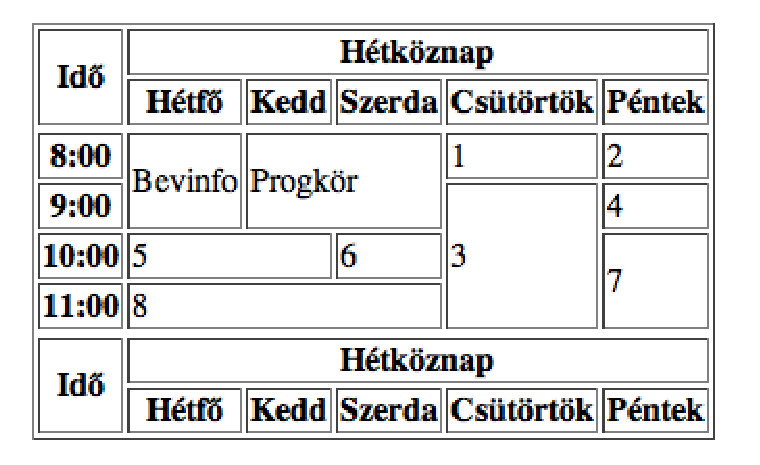
\includegraphics[scale=0.7]{html-table-view.eps}%
\end{center}%
  \caption{Az összetett táblázat (\ref{fig:html-table}.\ ábra) kinézete}%
  \label{fig:html-table-view}%
\end{figure}

A táblázatot a \texttt{table} elem jelöli, a sorokat pedig a \texttt{tr}. Egy
táblázatnak kétfajta cellája lehet, az egyik a fejléchez tartozik, ennek
megfelelően \texttt{th} a neve (table head), a másik az adatok tárolására
szolgál, ez a \texttt{td} (table data). Bár tipikusan az első pár sor a fejléc,
előfordulhat \texttt{th} elem a sorok elején is, akárcsak a láblécben.

Egy cella nem feltétlenül 1x1-es, hiszen nemegyszer össze kell fogni több
oszlopot a fejlécben, vagy éppen sort, ráadásul az adatrészben is
előfordulhatnak. Ha nem adjuk meg, hogy hány sornyi illetve oszlopnyi legyen,
akkor az alapértelmezett 1 értéket kapja, különben legalább az egyiket ki kell
írni. Tehát ha egy $n\times m$-es cellát szeretnénk megadni, ahol $n$ a sorok,
$m$ pedig az oszlopok számát jelöli, akkor azt a \texttt{rowspan} és
\texttt{colspan} attribútumokkal tehetjük meg a következőképpen (az összes nem
1x1-es lehetőséget felsorolva):

\begin{Verbatim}[frame=single]
<td colspan="m" rowspan="n">adat...</td>
<td rowspan="n" colspan="m">adat...</td>
<td rowspan="n">adat...</td>
<td colspan="m"">adat...</td>
\end{Verbatim}

\section{Formázás CSS-sel}\label{sec:html-css}
A \textsc{html}-t egy ideig használták formázásra is, mára azonban szinte csak
\textsc{css} kóddal határozzák meg az oldalak kinézetét. Ez utóbbi nagy előnye,
hogy a stílus (azaz a kinézet) és a tartalom különválik, így akár több
\textsc{html} oldal kinézetét is lehet befolyásolni egyetlen \textsc{css}
állomány módosításával. \Aref{fig:html-css-head}.\ ábrán látható módon lehet a
\textsc{html} dokumentumban megadni a stílust, valamint
\aref{fig:html-css-external}.\ ábrán látható módon lehet akár több külső
\textsc{css} állományt is használni. Természetesen a két megoldás együtt is
használható, például akkor, ha csak az adott oldalhoz kell stílust definiálni
-- bár még ekkor is jobb a külső fájl a könnyebb módosíthatóség és kezelhetőség
miatt.


\begin{figure}[tbh]
\begin{Verbatim}[frame=single]
<!DOCTYPE HTML PUBLIC "-//W3C//DTD HTML 4.0//EN">
<html>
  <head>
  <title>Bach's home page</title>
  <style type="text/css">
    body { 
      font-family: "Gill Sans", sans-serif;
      font-size: 12pt;
      margin: 3em; 
    }
  </style>
  </head>
  <body>
    <h1>Bach's home page</h1>
    <p>Johann Sebastian Bach was a prolific composer.</p>
  </body>
</html>
\end{Verbatim}
\caption{}
\label{fig:html-css-head}
\end{figure}

\begin{figure}[tbh]
\begin{Verbatim}[frame=single]
<!DOCTYPE HTML PUBLIC "-//W3C//DTD HTML 4.0.1//EN">
<html>
  <head>
  <title>Bach's home page</title>
  <style type="text/css">@import "system/default.css";</style>
  <link rel="stylesheet" type="text/css" href="system/tables.css"/>
  </head>
  <body>
    <p>Johann Sebastian Bach was a prolific composer.</p>
  </body>
</html>
\end{Verbatim}
\caption{}
\label{fig:html-css-external}
\end{figure}



Az azonosító lehet egyrészt a fent látható módon egy elem neve,
másrészt egy osztály, harmndrészt pedig egy azonosító. Az első már ismert, így
most tekintsük az utóbbi jettőt. Egy \textsc{html} elem tartozhat valamely
stílusosztályba, amelyet a \texttt{class} attribútum határoz meg, valamint lehet
egy egyedi azonosítója, amelyet a linkeknél említett \texttt{id} attribútum
határoz meg.

A példákban látható módon megadott \textsc{css} definíciókban szereplő azonosító
egy vagy több \textsc{html} elem nevét is tartalmazhatja, pl. \texttt{table.main
  tr.odd td \{...\}}, ami azt jelenti, hogy a \texttt{main} osztályba tartozó
\texttt{table} elemen belül valahol szerepel egy \texttt{odd} osztályú
\texttt{tr} elem, melyben egy \texttt{td} elem található. E \texttt{td} elem
(amely nem feltétlenül létezik, s ekkor a stílusdefiníció nem jut érvényre)
kinézetét befolyásolja. Lényeges, hogy itt nem szülő-gyerek, hanem
szülő-leszármazott (unoka stb.\ ugyanúgy lehet) viszonyról van szó, tehát a
\texttt{table} és \texttt{tr} elem között lehet például egy \texttt{tbody} elem
is, sőt a definíció a \texttt{td} elemben megadott másik táblázatbeli
\texttt{td} elemre is vonatkozik!

A Cascading Style Sheets elnevezés is innen ered, vízesésszerűen vonul végig az
adott beállítás az egyes elemeken. Ha egy általános elemre (pl.\ a
\texttt{td}-re) definiált valami, akkor annak specializált változataira (pl.\
adott stílusosztályba tartozókra: \texttt{td.first}) is vonatkozik az a
beállítás. Természetesen -- a legtöbb esetben -- ez felülbírálható a
specializált esetben is.

Lehet csak az adott \textsc{html} elemre vonatkozó stílusdefiníció, ha a
\texttt{style} attribútumot használjuk, mint például az \textsc{xhtml} 1.0
Transitional változatának \texttt{u} elemének megfelelő, 1.0 Strict és 1.1-es
változatában használható megoldás: \texttt{style="text-decoration: underline"}.

% Local Variables:
% fill-column: 80
% mode: latex
% End:
